\documentclass[12pt, letterpaper]{article}
\usepackage[titletoc,title]{appendix}
\usepackage{color}
\usepackage{booktabs}
\usepackage{caption}
\newcommand\fnote[1]{\captionsetup{font=small}\caption*{#1}}

\usepackage{float}

\usepackage[usenames,dvipsnames,svgnames,table]{xcolor}
\definecolor{dark-red}{rgb}{0.75,0.10,0.10} 
\usepackage[margin=1in]{geometry}
\usepackage[linkcolor=blue,
            colorlinks=true,
            urlcolor=blue,
            pdfstartview={XYZ null null 1.00},
            pdfpagemode=UseNone,
            citecolor={blue},
            pdftitle={UK Soft News}]{hyperref}

\usepackage{multibib}
\usepackage{geometry} % see geometry.pdf on how to lay out the page. There's lots.
\geometry{letterpaper}               % This is 8.5x11 paper. Options are a4paper or a5paper or other... 
\usepackage{graphicx}                % Handles inclusion of major graphics formats and allows use of 
\usepackage{amsfonts,amssymb,amsbsy}
\usepackage{amsxtra}
\usepackage{natbib}
\usepackage{longtable}

\usepackage{verbatim}
\setcitestyle{round,semicolon,aysep={},yysep={;}}
\usepackage{setspace}             % Permits line spacing control. Options are \doublespacing, \onehalfspace
\usepackage{sectsty}             % Permits control of section header styles
\usepackage{lscape}
\usepackage{fancyhdr}             % Permits header customization. See header section below.
\usepackage{url}                 % Correctly formats URLs with the \url{} tag
\usepackage{fullpage}             %1-inch margins
\usepackage{multirow}
\usepackage{rotating}
\setlength{\parindent}{3em}
\usepackage{subcaption}
\usepackage[T1]{fontenc}
%\usepackage{bm}
\usepackage{libertine}
%\usepackage{inconsolata}

\usepackage{chngcntr}

\title{\Large{Not News: Provision of Apolitical News in the British News Media}\footnote{Scripts behind the analysis can be downloaded at: \url{https://github.com/notnews/uk_not_news}. We are grateful to Kimberley Ortleb for assisting us in research. The paper benefitted from comments from Jamie Druckman, Daniel Stone, and Levi Boxell.}}

\author{Suriyan Laohaprapanon\thanks{Suriyan can be reached at: \href{mailto:suriyant@gmail.com}{\footnotesize{\texttt{suriyant@gmail.com}}}}\vspace{.5cm} \and Gaurav Sood\thanks{Gaurav can be reached at \href{mailto:gsood07@gmail.com}{\footnotesize{\texttt{gsood07@gmail.com}}}}}

\date{\vspace{.5cm}\normalsize{\today}}

\begin{document}
\maketitle

\begin{comment}

setwd(paste0(githubdir, "uk_not_news/ms"))
tools::texi2dvi("not_news_uk.tex", pdf = TRUE, clean = TRUE) 
setwd(githubdir)

\end{comment}

\begin{abstract}
\noindent What proportion of news is soft news? What proportion of articles published by a news outlet is about dining, travel, fashion, cooking, celebrity scandals, and other such things? Using a corpus of $\sim$ 5.4M web pages from 276 news outlets in the U.K. spanning 2003--2015, we estimate the provision of soft news on online news outlets. To measure soft news, we build a supervised model using text from articles whose URL structure provides a clear indication of the type of content. We validate the success of the classifier by hand coding 1,000 articles---the error rate is about 12\%. Using the classifier, we find that about 39\% of the articles are about topics other than public affairs. 
\end{abstract}

\clearpage
\doublespacing

News media is justly seen as vital to a healthy democracy. Consumption of news causes a wide variety of virtuous outcomes, from political participation to political accountability \citep{gentzkow2015, oberholzer2006media, snyder2008press, stromberg2004radio}. These benefits doubtlessly stem from consumption of policy- or policy-maker (or enforcer) relevant information, as opposed to say, news about cooking, fashion, and such \citep[see, for instance,][]{prior2003}. Thus, to assess the health of the fourth estate, it is vital to understand how much of the news is broadly about public affairs, and how much of it is about cooking, sports, travel, movie reviews, fashion, and such, and how that may be changing over time.

To answer this important question, we build on prior work on measurement of public affairs news, modifying the previously proposed method in a small but important way to reduce generalization error. We then apply the method to estimate how much of the British news is broadly about public affairs using a corpus of $\sim$ 5.4M web pages from 276 separate news outlets in the U.K. spanning 2003--2015. 

We measure soft news using a classifier based on keywords in the URL \citep{bakshy2015exposure, flaxman2016filter}. To ensure that the model generalizes, we use the entire story text but only rely on bigrams and trigrams that are common across outlets. The out of sample precision and recall of our model is about 88\% each. To estimate generalization error, we validate the success of the classifier by getting manually coded labels for 1,000 articles. The generalization error is very close to our model estimates at about 12\%.

We use the model to classify our corpus. We find that about 39\% of all the articles are about non-public affairs. When we group articles by outlet, we find that, on average, 45\% of the articles in an outlet are about cooking, travel, entertainment, and similar such things. 

\section*{Incentives for Soft News}
What explains the provision of soft news on news websites? The conventional story goes something like this. Profit-maximizing private companies control many of the news media outlets. And to the extent that provision of soft news increases profits, for instance, by increasing the size of the audience or by reducing production costs, news media outlets provide soft news. But the story is a bit more nuanced. To explore the issues in depth, we start by looking at demand and segue into supply-side issues.

Data suggest that there is strong demand for soft news \citep{arceneaux2013changing, barnhurst1997, flaxman2016filter, guess2016media}. But what explains demand for soft news? People probably want soft news because it entertains them. Another less obvious reason why people may want soft news is that it is good fodder for conversation. Politics is too controversial a topic in many social settings. And celebrities, popular television shows, etc. are less controversial, widely known facets of society that people can discuss without fear of offending others. Because of such reasons and reasons like these, apolitical news is popular. And in a capitalist media system \citep{curran2009media}, we expect customer tastes to matter. Much like \citet{gentzkow2006drives} show that customer tastes explain partisan bias, we suspect customer tastes also explain the provision of soft news.

We also expect owner tastes to matter less over time. The conventional wisdom around the `oversupply' of political news in the 50s and 60s on network television in the U.S. is that the television network owners thought it in good taste to provide it. However, public listing of many of the media companies has likely changed owners palate (incentives), with a taste for profit replacing any public-minded instincts. Aside from that, deregulation of television, for instance, the 1996 Telecommunications Act in the U.S., the advent of Internet, which largely doesn't impinge on public resources, in lieu of which the government could regulate, has reduced government's role in shaping television content. 

But this is just one part of the story. The other part is the collapse of the two major streams of newspaper revenue: 1) newspaper sales---people have become less inclined to pay for news post `free' access to content, and 2) paid classifieds---today, services like Craigslist and Facebook provide a cheaper (free) way to post classifieds. And to address the revenue shortfall, news media have looked to cut costs. 

To reduce costs, news media have a lot of levers in hand, from making more extensive use of wire stories to reducing the number of foreign news bureaus \citep{schudson2005, shanor2013} to reducing the number journalists on staff to forcing journalists to produce more news articles (words, minimally) per week to turning to freelancers for reporting. The switch to soft news is likely part of the same strategy. News about celebrities and turkey contests is cheaper to produce than sending a journalist to Pakistan. And news media may substitute apolitical news for political news as a way to respond to lower revenues \citep{cage2012trash, davis1998new, kalb1998}.

When faced with lower revenues and financial pressures, newspapers can respond not just by finding cheaper ways to produce existing content (at lower quality), reducing, or replacing the content, but by also adding to it. For instance, newspapers may add a `lifestyle' section as a way to lure new customers (and keep old ones) without adding significantly to the costs. The reason for that is as follows. Easily detachable section based layout allows newspapers to cater to multiple audiences at the same time. (Television and radio, by contrast, are different. Tuning into television means that you and everyone else in the earshot is exposed to the channel you are tuned into unless, of course, you listen using headphones.) A surfeit of web-enabled devices means that news websites are similar to paper versions in that they can also simultaneously cater to multiple audiences. For instance, the politically interested Democrat in the family may go to \href{huffingtonpost.com}{huffingtonpost.com} for reading up on the latest Republican outrage, while the celebrity-obsessed member of the family may go there for the latest gossip. 

In all, strong demand for soft news, declining regulation, declining influence of owner tastes, and declining revenue plausibly contribute to provision of soft news on news sites.

\section*{Data and Measurement}
Our corpus has $\sim 5.73M$ de-duped web pages. We filter on years for which we have more than 10,000 web pages. It leaves us with $\sim 5.71M$  spanning 2003--2015. Next, we drop web pages for which we don't have a URL. Doing that leaves us with about $\sim 5.44M$ web pages. For about $2K$ articles, we can't parse the domain name mostly because they have an IP address than a domain. We remove these web pages as well. This leaves us with 5,442,931 articles. Before we cull the data further, we clean outlet labels. 

To produce clean outlet labels, we start by stripping leading and trailing spaces in outlet names. Next, we manually sift through the domains and combine domains that track the same source. Lastly, we manually create outlet names based on domain name and source name from the metadata of the web pages. We use these outlet labels to filter on sources with 1,000 or more web pages. (We feel that we would have too little data on other outlets to make reliable judgments.) This leaves us with 5,392,953 articles spanning 276 outlets. This serves as our final dataset. Appendix \ref{si_media_sum_uk} provides a summary of the data including the number of transcripts per outlet, and the range of dates for which we have the data. (To better understand the limitations of the sample, we plot the total number of web pages per outlet per year, and tally other things like weeks with zero transcripts per source, in the \href{https://github.com/not_news/uk_not_news/blob/master/scripts/01_subset_summarize_uk_news_media_data_by_label.ipynb}{Jupyter Notebook}.)

To measure soft news, we use machine learning.  We start by taking a random sample of 1M news articles from our final dataset. Then, following \citet{bakshy2015exposure} and \citet{flaxman2016filter}, we use keywords in the URL to code the content of the web pages. In particular, after manually inspecting a large random sample, we label all URLs that match the following regular expression as political news:

\begin{quote}
politi|world|national|uk-news|scottish-news|news-eu|state|local|elect|vote|govern|\\
campaign|war|polic|econ|unemploy|energy|educa|healthcare|immigration
\end{quote}

\noindent And we label all URLs which match the following regular expression as soft news: 
\begin{quote}
sport|football|entertainment|culture|arts|fashion|style|lifestyle|life-style|leisure|\\
celeb|movie|music|gossip|food|travel|horoscope|weather|gadget
\end{quote}

Given that it is technically possible for a URL to have both sets of keywords, we further limit ourselves to URLs where the categorization is unique. We code the category of all other URLs as missing. This leaves us with a sample of 372,163 articles. We pre-process the news articles, lemmatizing, removing `stop words,' and punctuation, losing all words less than two characters long, and converting all the words to lower case. We further assume a 1-, 2- Markov model of language, storing just frequency of bi-grams and tri-grams and removing order information. (See \citet{gentzkow2010} and \citet{MartinYurukoglu2014}, among others who have used similar assumptions in modeling similar text.) For lower generalization error and for learning a model that isn't source specific, we only keep bi- and tri-grams that appear in 50 or more outlets. This leaves us with a vocabulary of 46,711 tokens. Further filtering on tokens that appear at least 100 times leaves us with a vocabulary size of 37,582. 

Next, we split the data into train (80\%) and test (20\%), and train a regularized Logistic Regression classifier \citep{zou2005regularization} on the training set, using cross-validation to pick the appropriate $\lambda$. Table \ref{tab:url_conf_matrix} presents out of sample performance of the model. The classifier is fairly accurate, correctly classifying 89\% of the apolitical articles out of sample.

\begin{table}[!htb]
\centering
\caption{Out-of-sample Performance of the Model} 
\label{tab:url_conf_matrix}
\begin{tabular}{lcccc}
\hline
labels & precision   &  recall  &   f1-score  &   support \\
\hline
Soft News      & 0.89    &   0.87    &   0.88   &    35,912 \\
News          & 0.86    &   0.90    &   0.88   &    38,521 \\
\hline
\end{tabular}
\end{table}

To further validate the model, we tabulate the top 100 predictors of news and soft news in Table \ref{tab:top_100_hard} and Table \ref{tab:top_100_soft} respectively. The tables make for a reassuring reading. The top predictors of news include bigrams and trigrams like ``nation news,'' ``war crime,'' ``helmand provinc,'' ``mr obama,'' ``mr brown,'' etc. And the top predictors of soft news include bigrams and trigrams like ``food drink,'' ``britney spear,'' ``manchest unit,'' ``box offic,'' ``aston villa,'' etc.  

\singlespacing

% latex table generated in R 3.5.2 by xtable 1.8-3 package
% Thu Jan 24 20:00:33 2019
\begingroup\small
\begin{longtable}{p{0.3\textwidth}p{0.3\textwidth}p{0.3\textwidth}}
\caption{Top 100 Predictors of Hard News} \\ 
  \hline
  \hline
nation news & spokeswoman said & play video \\ 
  comment new & war crime & helmand provinc \\ 
  report abus & end quot & secondari school \\ 
  local news & report said & northern rock \\ 
  gordon brown & report problem & mr obama \\ 
  comment articl & appear press & peopl die \\ 
  prime minist & view express & local elect \\ 
  polic offic & presidenti elect & local newspap \\ 
  barack obama & polic investig & print page \\ 
  comment post & mr brown & govern said \\ 
  person use & media report & debat issu \\ 
  kill peopl & news agenc & polit parti \\ 
  polic said & ministri defenc & said http \\ 
  gener elect & said mr & parti leader \\ 
  quot http & nation award & site http \\ 
  polic station & billion euro & went miss \\ 
  peopl kill & told bbc & oil ga \\ 
  comment http & tori leader & secur forc \\ 
  foreign minist & sinn fein & vladimir putin \\ 
  offici said & polic warn & campaign launch \\ 
  higher educ & spokesman said & west bank \\ 
  press associ & comment say & inform http \\ 
  liber democrat & offici say & poll station \\ 
  anyon inform & antisoci behaviour & european elect \\ 
  consid action & council elect & polic chief \\ 
  news stori & lib dem & busi award \\ 
  unit kingdom & opposit leader & award ceremoni \\ 
  local govern & mp expens & defenc minist \\ 
  media group & gener secretari & minist alex salmond \\ 
  hillari clinton & stab death & nuclear power \\ 
  add comment & death toll & al qaida \\ 
  shot dead & alistair darl & industri action \\ 
  scottish govern & labour parti &  \\ 
  crown court & share view &  \\ 
   \hline
\hline
\label{tab:top_100_hard}
\end{longtable}
\endgroup


\clearpage
% latex table generated in R 3.5.2 by xtable 1.8-3 package
% Thu Jan 24 20:00:33 2019
\begingroup\small
\begin{longtable}{p{0.3\textwidth}p{0.3\textwidth}p{0.3\textwidth}}
\caption{Top 100 Predictors of Not News} \\ 
  \hline
  \hline
relat articl & food drink & red card \\ 
  email text & start season & defend champion \\ 
  larg section & alex mcleish & debut album \\ 
  law order & leagu divis & ryder cup \\ 
  premier leagu & tv radio & european tour \\ 
  email friend print & west brom & art centr \\ 
  friend print page & real madrid & look like \\ 
  end season & offic uk & apo apo \\ 
  friend print & head coach & think say \\ 
  live council & autumn statement & manchest unit \\ 
  champion leagu & daili telegraph & london irish \\ 
  tv news & new manag & young player \\ 
  manchest citi & transfer window & person view \\ 
  second half & ipswich town & food industri \\ 
  aston villa & knee injuri & royal ascot \\ 
  celebr year & super leagu & tell stori \\ 
  grand prix & west indi & film festiv \\ 
  box offic & britney spear & follow twitter \\ 
  food safeti & arsen wenger & final round \\ 
  travel site & feel like & classic music \\ 
  debt crisi & celebr birthday & apo new \\ 
  accrington stanley & hemel hempstead & sound like \\ 
  blackburn rover & new film & music festiv \\ 
  west ham & phone hack & win game \\ 
  london olymp & ami winehous & real life \\ 
  britain apo & footbal leagu & kevin pietersen \\ 
  new album & gold cup & road rail \\ 
  counti championship & score goal & sign new \\ 
  heineken cup & premier divis & fa cup \\ 
  oliv oil & run time & cardiff citi \\ 
  footbal associ & birmingham citi & littl bit \\ 
  oxford unit & stamford bridg & financi crisi \\ 
  latest news & food bank &  \\ 
  leisur centr & today apo &  \\ 
   \hline
\hline
\label{tab:top_100_soft}
\end{longtable}
\endgroup


\doublespacing

\section*{Results}
We start by describing the overall provision of soft news. We treat each article as an observation, and plot the density of soft news (see Figure \ref{fig:agg_density}).  Nearly 39\% of the articles are about cooking, sports, lifestyle, and such topics. This number, however, may not be a good guide to provision of soft news across outlets. For instance, if the least political outlets are also the most prolific, treating each article the same would lead us to think that the average is higher. So, next, we tallied the proportion of soft news stories in each of the outlets. The average percentage of soft news stories per outlet is nearly 45\% while the median is 46\% and the 25th percentile is an astonishing 38\%. \textit{Haringey Independent} tops the charts with 78.3\% of its articles being soft news. In all, it appears that a hefty proportion of news articles across outlets are about soft news.

\begin{figure}[!htbp]
\centering
\caption{Share of Soft News Across Outlets}
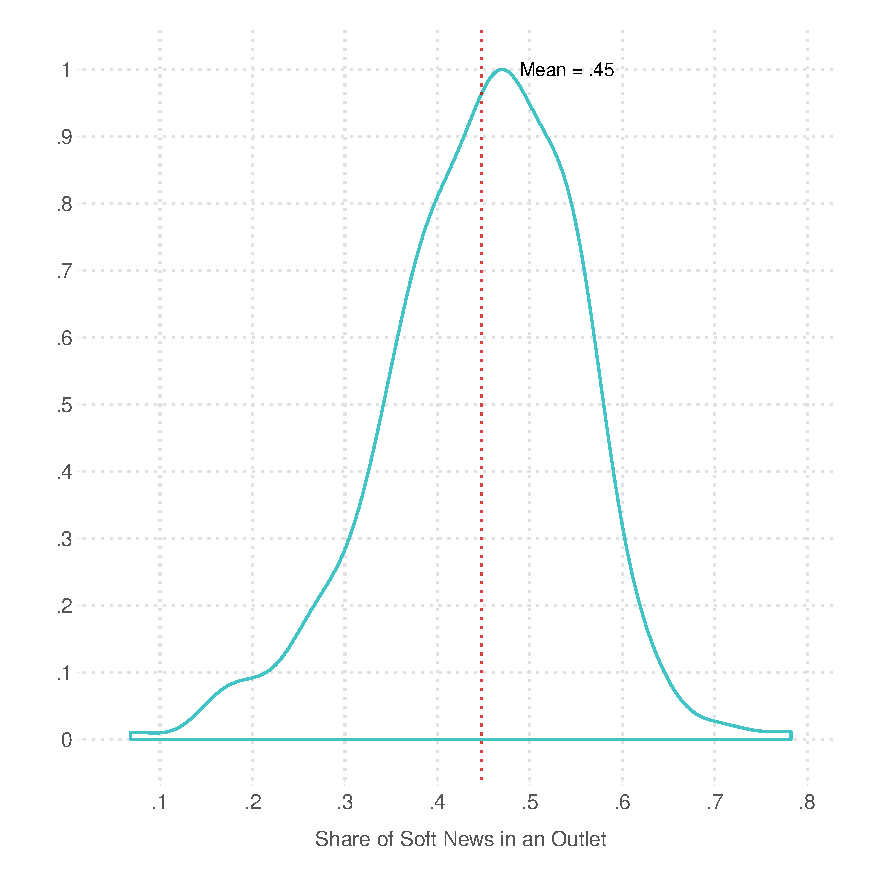
\includegraphics[scale=.9]{../figs/uk_not_news_by_outlet.pdf}
\label{fig:agg_density}
\end{figure}

Figure \ref{fig:uk_dot_plot} highlights provision of soft news in some prominent outlets. Expectedly, the tabloid \textit{The Daily Star} takes the top spot with 66\%. Somewhat surprisingly, about 48\% the articles on BBC are soft news. The commensurate number for \textit{The Guardian} is 41\%. 

\begin{figure}[!htbp]
\centering
\caption{Share of Soft News Across Prominent Outlets}
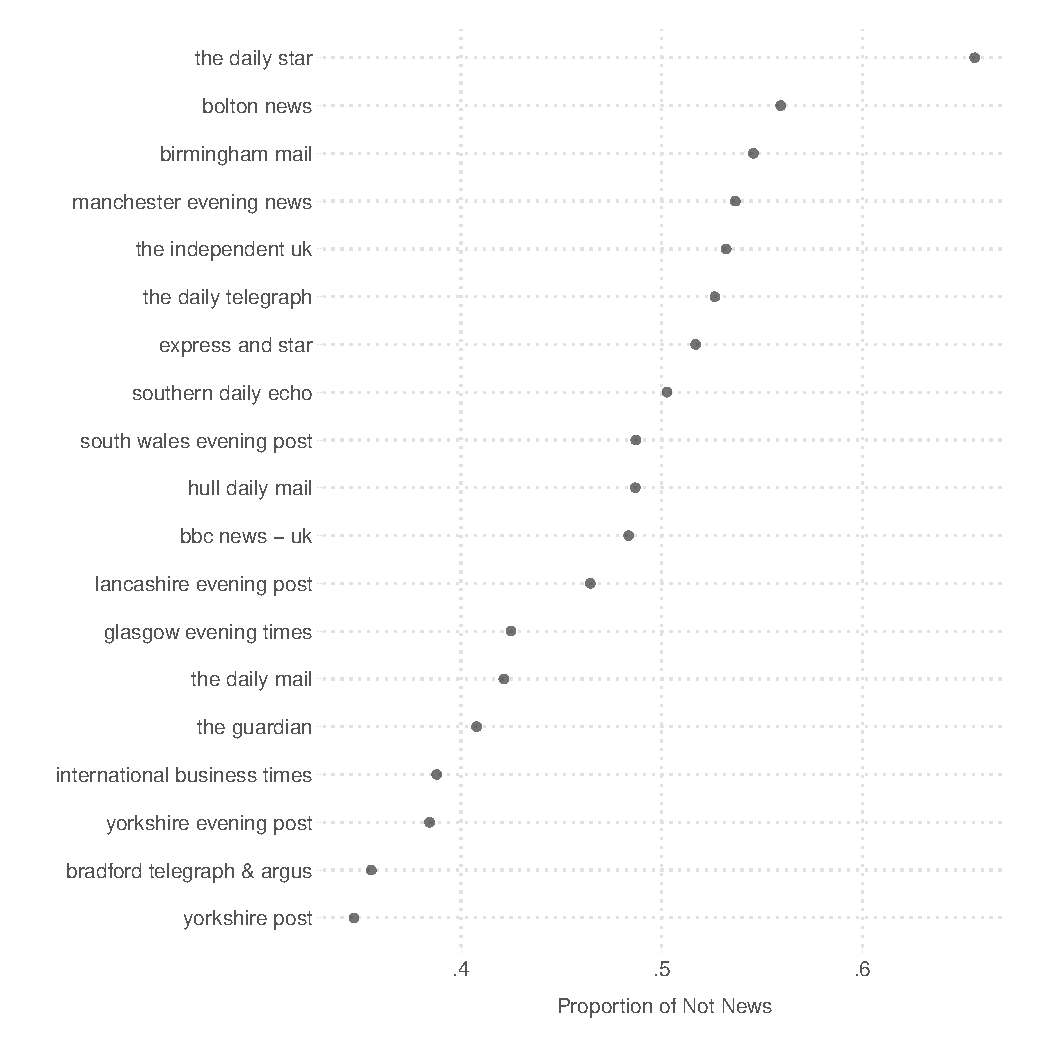
\includegraphics[scale = .9]{../figs/uk_not_news_by_outlet_main_dotplot.pdf}
\label{fig:uk_dot_plot}
\end{figure}

Splitting by domain rather than outlet doesn't change the complexion of the results (see Figure \ref{fig:agg_density_domain}). The average proportion of soft news across domains is 46\%. The median is 45\%, and the maximum is 74\% (for \url{chroniclelive.co.uk}).

Next, we estimate the provision of soft news over time. To estimate how the provision of soft news is changing over time, we start by regressing probability an article is soft news on year rescaled to range from 0 (2003) to 1 (2015) and one-hot-encoded outlets. This gives us an estimate of `average' change assuming that the outlet mix of our sample remains the same. The results suggests that over time the proportion of soft news has increased by roughly 8\%. 

To explicitly look at within outlet trends, we subset on rows for each source and estimate trend for each outlet by regressing probability of a soft news article on year, rescaled as above. We then average coefficients over all these regressions and then estimate how on the provision of soft news is changing across outlets on average. This specification gives each outlet equal weight. If we do that, we get an estimate of about 1\% increase in soft news over time.

\section*{Discussion}
Near tautologically, lower the political content, lesser the opportunity to learn something relevant for political decision making \citep{prior2003, curran2009media}, and greater the opportunity to be distracted. This is not to say that news about celebrities, entertainment, food, and travel do not affect people's political attitudes and beliefs. But it is to say that people will not be better at holding politicians accountable or be better able to execute their preferences, if they consume more soft news. In this article, we shed light on measuring soft news and describing the privision of soft news. And in shedding light on this important measure of the quality of news, the article contributes to the literature on media effects.

\clearpage
\normalfont
\normalsize
\doublespace%
\bibliographystyle{apsr}
\bibliography{not_news}  

\clearpage
\appendix
\renewcommand{\thesection}{SI \arabic{section}}
\setcounter{table}{0}\renewcommand\thetable{\thesection.\arabic{table}}  
\setcounter{figure}{0}\renewcommand\thefigure{\thesection.\arabic{figure}}
\counterwithin{figure}{section}

\section{Summary of the Media Data}
\label{si_media_sum_uk}
A complete list of domains from which we collected articles, the range of dates for which we have data from each, and the number of articles.

\scriptsize
% latex table generated in R 3.5.2 by xtable 1.8-3 package
% Fri Jan 25 20:37:48 2019
\begingroup\tiny
\begin{longtable}{p{0.45\textwidth}p{0.15\textwidth}p{0.15\textwidth}p{0.1\textwidth}}
\caption{Summary of the Media Data} \\ 
  \hline
Name & From & To & No. of Transcripts \\ 
  \hline
24dash & 13504 & 15446 & 43652 \\ 
  A World to Win Blogs & 15345 & 16342 & 1549 \\ 
  Agra-Net.com & 13600 & 16150 & 14391 \\ 
  Al-Sharq Al-Awsat & 13260 & 15762 & 35672 \\ 
  Alliance for Workers' Liberty & 12079 & 16259 & 1781 \\ 
  Ananova & 13618 & 15607 & 86893 \\ 
  Andover Advertiser & 13600 & 16307 & 7540 \\ 
  Ayrshire Post & 13588 & 15886 & 9202 \\ 
  BBC News & 12101 & 16470 & 120772 \\ 
  Bakery and Snacks & 13711 & 15924 & 3807 \\ 
  Ballyclare Gazette & 14420 & 16086 & 1246 \\ 
  Ballymena Times & 13851 & 15526 & 4338 \\ 
  Ballymoney Today & 13119 & 15014 & 25633 \\ 
  Banbridge Leader & 13167 & 15526 & 34811 \\ 
  Banbury Guardian & 13522 & 15883 & 37290 \\ 
  Barking and Dagenham Post & 13033 & 14875 & 6193 \\ 
  Barnet Times & 13719 & 15321 & 33555 \\ 
  Barnsley Chronicle & 13525 & 15739 & 3978 \\ 
  Basingstoke Gazette & 13287 & 16263 & 25255 \\ 
  Beccles and Bungay Journal & 13581 & 14879 & 5986 \\ 
  Bedford Times and Citizen & 12555 & 15884 & 24715 \\ 
  Belfast Media & 13637 & 15232 & 45231 \\ 
  Belfast Telegraph & 13001 & 15860 & 263918 \\ 
  Belfast Today & 13676 & 15525 & 3584 \\ 
  Berwick Today & 13354 & 15530 & 6696 \\ 
  Bexhill Observer & 13812 & 15878 & 18234 \\ 
  Birmingham Mail & 14049 & 16259 & 80567 \\ 
  Bishop's Stortford Citizen & 13592 & 14267 & 20120 \\ 
  Blackburn Citizen & 13522 & 16213 & 36210 \\ 
  Blackpool Citizen & 13216 & 16239 & 11621 \\ 
  Blackpool Today & 13578 & 14986 & 13362 \\ 
  Bognor Today & 13759 & 16470 & 21769 \\ 
  Bolton News & 13593 & 16171 & 92852 \\ 
  Border Telegraph & 13046 & 15714 & 1770 \\ 
  Borehamwood and Elstree Times & 13594 & 16259 & 67130 \\ 
  Boston Standard & 12823 & 15525 & 12871 \\ 
  Bournemouth Daily Echo & 15338 & 16162 & 7350 \\ 
  Bracknell Times & 13417 & 15867 & 10033 \\ 
  Bradford Telegraph and Argus & 15464 & 16213 & 15105 \\ 
  Brechin Today & 13055 & 15529 & 18950 \\ 
  Brighton Evening Argus & 14730 & 16319 & 9108 \\ 
  Bromley Times & 13748 & 14946 & 2829 \\ 
  Buckingham Today & 13287 & 15396 & 44622 \\ 
  Bucks Free Press & 15340 & 16259 & 6195 \\ 
  Bucks Herald & 12508 & 15883 & 13226 \\ 
  Burnley Express & 13077 & 15524 & 11175 \\ 
  Bury Free Press & 13578 & 15880 & 15140 \\ 
  Bury Times & 13561 & 16263 & 46248 \\ 
  Business Weekly - UK & 14043 & 14984 & 1485 \\ 
  Buxton Advertiser & 13615 & 15524 & 118757 \\ 
  Cambridge Evening News & 12325 & 15600 & 39484 \\ 
  Cambs Times & 13588 & 16259 & 12758 \\ 
  Chard and Ilminster News & 13667 & 16213 & 12669 \\ 
  Cheshire Online & 12467 & 15883 & 54587 \\ 
  Chester Evening Leader & 13522 & 14442 & 2201 \\ 
  Chester Standard & 13588 & 15876 & 25986 \\ 
  Chichester Observer & 13713 & 15526 & 25994 \\ 
  Chingford Guardian & 13588 & 14077 & 5883 \\ 
  Chorley Citizen & 13422 & 16258 & 20925 \\ 
  Clitheroe Today & 14373 & 15021 & 2919 \\ 
  Colchester Daily Gazette & 14083 & 16470 & 28158 \\ 
  Cornish Guardian & 14344 & 16147 & 16971 \\ 
  Country Life & 13182 & 15425 & 2825 \\ 
  County Times & 13585 & 15866 & 1590 \\ 
  Coventry Telegraph & 13635 & 15883 & 24206 \\ 
  Crawley Observer & 13599 & 15883 & 15810 \\ 
  Croydon Guardian & 13588 & 16307 & 19321 \\ 
  Cumberland and Westmorland Herald & 13546 & 15883 & 2134 \\ 
  Daily Express & 13522 & 15742 & 19656 \\ 
  Daily Post & 13522 & 16470 & 66240 \\ 
  Daily Record & 13634 & 15552 & 51530 \\ 
  Darlington and Stockton Times & 13588 & 16213 & 22180 \\ 
  Derby Evening Telegraph & 15338 & 15948 & 21609 \\ 
  Derbyshire Times & 13966 & 15525 & 4600 \\ 
  Derry Journal & 14420 & 15878 & 3218 \\ 
  Diss Mercury & 13825 & 16352 & 4089 \\ 
  Doncaster Free Press & 13475 & 15523 & 9354 \\ 
  Donegal News & 13567 & 13868 & 2426 \\ 
  Driffield Times and Post & 13402 & 15887 & 6437 \\ 
  Dromore Leader & 13202 & 15879 & 1700 \\ 
  Dunmow Broadcast & 15433 & 16385 & 1237 \\ 
  EUbusiness & 15340 & 16259 & 6505 \\ 
  Ealing Times & 13588 & 16213 & 4339 \\ 
  East Anglian Daily Times & 13588 & 14609 & 18578 \\ 
  East Lothian Courier & 13524 & 16162 & 5248 \\ 
  Eastbourne Herald & 13533 & 14609 & 9833 \\ 
  Eastern Daily Press & 13588 & 16259 & 27908 \\ 
  Eastwood Advertiser & 12832 & 15886 & 19548 \\ 
  Echo - Essex News and Sports & 13588 & 16307 & 26522 \\ 
  Edgware and Mill Hill Times & 13104 & 15583 & 14259 \\ 
  Ely Standard & 13588 & 16386 & 5511 \\ 
  Environmental Agency UK & 14157 & 16157 & 1514 \\ 
  Epping Forest Guardian & 13588 & 14077 & 5849 \\ 
  Epsom Guardian & 13588 & 16212 & 12412 \\ 
  Essex Chronicle & 14306 & 16050 & 7225 \\ 
  Evening Gazette & 13590 & 14077 & 11605 \\ 
  Evening Star (Ipswich) & 13474 & 16470 & 40262 \\ 
  Evening Telegraph & 13599 & 15391 & 5846 \\ 
  Express and Star & 13990 & 16470 & 30510 \\ 
  Farmers Guardian & 13753 & 16470 & 19275 \\ 
  Farmers Weekly Interactive & 13199 & 16255 & 24106 \\ 
  Farming UK & 14313 & 16415 & 6405 \\ 
  Food Naviagtor & 13598 & 14601 & 2846 \\ 
  Food Navigator & 13724 & 16470 & 5923 \\ 
  Fruit Net (UK and Germany) & 14587 & 15637 & 1653 \\ 
  Gazette and Herald & 13797 & 16213 & 12849 \\ 
  Gazette Live & 13074 & 15824 & 19382 \\ 
  Glasgow Evening Times & 13746 & 15883 & 7032 \\ 
  Gloucestershire County Gazette & 13764 & 15739 & 3425 \\ 
  Google News & 14695 & 16470 & 7471 \\ 
  Grantham Today & 13634 & 15874 & 13578 \\ 
  Great Yarmouth Mercury 24 & 13958 & 14609 & 7010 \\ 
  Grimsby Telegraph & 15340 & 15948 & 3331 \\ 
  Guardian Series & 14083 & 16307 & 91419 \\ 
  Hackney Gazette & 13047 & 15719 & 4399 \\ 
  Hampshire Chronicle & 13294 & 16259 & 13456 \\ 
  Hampstead and Highgate Express & 13545 & 16470 & 3786 \\ 
  Harborough Mail & 13588 & 15918 & 4551 \\ 
  Haringey Independent & 12263 & 15583 & 6300 \\ 
  Harlow Citizen & 13589 & 14224 & 1862 \\ 
  Harrow Times & 12431 & 16259 & 14132 \\ 
  Hartlepool Mail & 12346 & 15846 & 35403 \\ 
  Hemel Today & 13490 & 15875 & 19242 \\ 
  Hendon and Finchley, Barnet and Potters Bar, and Edgeware and Mills Hill Times & 13719 & 16213 & 3155 \\ 
  Herald and Post & 13588 & 14609 & 26902 \\ 
  Hertferdshire Mercury & 13753 & 16259 & 11072 \\ 
  Hexham Courant & 13399 & 16469 & 5518 \\ 
  Highland News & 13587 & 16212 & 4900 \\ 
  Hillingdon Times & 13587 & 15392 & 6198 \\ 
  Horncastle News & 12165 & 15947 & 36426 \\ 
  Horticulture Week & 15342 & 15636 & 1277 \\ 
  Hucknall Dispatch & 13585 & 15948 & 7450 \\ 
  Hull Daily Mail & 15341 & 15947 & 18489 \\ 
  Hunts Post & 13588 & 16399 & 5375 \\ 
  IC Newcastle & 13384 & 15748 & 34137 \\ 
  IC Teesside & 13444 & 14609 & 7586 \\ 
  ITN News & 13587 & 14609 & 37944 \\ 
  Ilford Recorder & 13565 & 16370 & 5925 \\ 
  Ilkeston Advertiser & 12257 & 15948 & 5353 \\ 
  Ilkley Gazette & 13523 & 15583 & 5640 \\ 
  Impartial Reporter & 15337 & 15714 & 1981 \\ 
  In the News & 13450 & 15685 & 36422 \\ 
  Inspire Magazine & 13796 & 15461 & 2461 \\ 
  Insurance Insight & 15618 & 16048 & 1289 \\ 
  International Business Times & 13997 & 16470 & 85135 \\ 
  Isle of Wight County Press & 13797 & 16327 & 13338 \\ 
  Journal Live & 13772 & 15883 & 20003 \\ 
  Kenilworth Weekly News & 13885 & 15924 & 8798 \\ 
  Kingston Guardian & 13588 & 16307 & 12284 \\ 
  Lancashire Evening Post & 13495 & 16162 & 40491 \\ 
  Lancashire Evening Telegraph & 14799 & 16193 & 7987 \\ 
  Lancashire Telegraph & 12500 & 16259 & 64429 \\ 
  Leamington Observer & 13909 & 16470 & 2397 \\ 
  Leicester Mercury & 14495 & 15949 & 20944 \\ 
  Leicester Sound & 13600 & 14152 & 1855 \\ 
  Leigh Journal & 13277 & 16307 & 19456 \\ 
  Lincolnshire Echo & 15340 & 16056 & 11839 \\ 
  Lisburn Today & 13196 & 14609 & 9319 \\ 
  Liverpool Daily Post & 13522 & 14609 & 39071 \\ 
  Liverpool Echo & 13690 & 15775 & 33691 \\ 
  Local London & 13913 & 16263 & 13305 \\ 
  London Turkish Gazette & 14157 & 15470 & 1190 \\ 
  Louth Leader & 13580 & 15926 & 35502 \\ 
  Lurgan Mail & 13146 & 15947 & 5980 \\ 
  Luton News Herald and Post & 15340 & 15525 & 1526 \\ 
  Lynn News & 13581 & 15525 & 4211 \\ 
  Manchester Evening News & 12074 & 15728 & 35909 \\ 
  Mansfield Today & 13588 & 13747 & 7490 \\ 
  Mansfield and Ashfield Chad & 13604 & 16462 & 5797 \\ 
  Matlock Mercury & 13306 & 15947 & 3311 \\ 
  Melton Times & 13461 & 16052 & 5890 \\ 
  Metro - London & 13587 & 16470 & 43471 \\ 
  Morning Star Online & 13522 & 15946 & 9942 \\ 
  Morpeth Herald & 13489 & 15922 & 3434 \\ 
  Newbury Today & 12934 & 16328 & 5638 \\ 
  Newham Recorder & 13517 & 16370 & 5246 \\ 
  Newry Democrat & 12054 & 16259 & 1948 \\ 
  News and Star & 12615 & 16318 & 32852 \\ 
  News Guardian & 15711 & 15883 & 1561 \\ 
  News Post Leader & 13594 & 15885 & 12058 \\ 
  News Shopper & 13588 & 16259 & 10184 \\ 
  News Wales & 13585 & 15494 & 2688 \\ 
  NewsNet Scotland & 15177 & 16331 & 4954 \\ 
  North Tyneside Today & 13593 & 13878 & 2140 \\ 
  North Wales Chronicle & 13574 & 16328 & 4874 \\ 
  North-West Evening Mail & 13594 & 16469 & 9273 \\ 
  Northampton Chronicle and Echo & 13588 & 16470 & 19851 \\ 
  Northamptonshire Evening Telegraph & 13588 & 15490 & 3341 \\ 
  Northern Ireland Executive & 15350 & 16470 & 5630 \\ 
  Northumberland Gazette & 13633 & 15921 & 5219 \\ 
  Norwich Evening News 24 & 13528 & 16470 & 33174 \\ 
  Nottingham Post & 15340 & 15948 & 23000 \\ 
  Ongar Guardian & 13588 & 13879 & 2980 \\ 
  Open Democracy & 13838 & 15516 & 1031 \\ 
  Ormskirk Advertiser & 12641 & 16155 & 7496 \\ 
  Oxford Mail & 13227 & 16470 & 47232 \\ 
  PR Newswire & 13798 & 15930 & 5603 \\ 
  Paisley Daily Express & 13746 & 15692 & 18870 \\ 
  Pendle Today & 13301 & 15524 & 10778 \\ 
  Peterborough Evening Telegraph & 13559 & 15834 & 20896 \\ 
  Petersfield Post & 12634 & 16094 & 5353 \\ 
  Plymouth Herald & 15498 & 15948 & 3350 \\ 
  Preston Citizen & 13158 & 16305 & 2677 \\ 
  Reading Post & 13712 & 16469 & 18122 \\ 
  Redhill and Reigate Life & 13588 & 16462 & 3209 \\ 
  Retford Guardian & 13475 & 15948 & 4441 \\ 
  Reuters AlertNet & 13434 & 15818 & 91444 \\ 
  Richmond and Twickenham Times & 13588 & 16307 & 5695 \\ 
  Ripley and Heanor News & 13690 & 15947 & 3319 \\ 
  Rochdale Observer & 12947 & 15724 & 1921 \\ 
  Romsey Advertiser & 13322 & 16304 & 2242 \\ 
  Royston Crow & 13579 & 16469 & 5859 \\ 
  Rutland News & 13587 & 13873 & 1341 \\ 
  Rutland Times & 13599 & 15943 & 8563 \\ 
  Saffron Walden Reporter & 13579 & 16385 & 3920 \\ 
  Sale and Altrincham Messenger & 13594 & 16213 & 5606 \\ 
  Scotsman & 12484 & 15876 & 46782 \\ 
  Scunthorpe Telegraph & 15340 & 15948 & 9194 \\ 
  Sheffield Today & 13401 & 15525 & 13699 \\ 
  Skegness Today & 13531 & 13878 & 4168 \\ 
  SkyNews & 12075 & 16213 & 23848 \\ 
  Slough and South Bucks Observer & 15340 & 15886 & 2514 \\ 
  Somerset County Gazette & 15340 & 16322 & 5015 \\ 
  South London Press & 13584 & 13977 & 7848 \\ 
  South Wales Argus & 13587 & 15392 & 3698 \\ 
  South Wales Evening Post & 15706 & 16470 & 11987 \\ 
  Southern Daily Echo & 13218 & 16325 & 68458 \\ 
  Spalding Guardian & 15319 & 15876 & 4328 \\ 
  Spalding Today & 13585 & 14609 & 8977 \\ 
  St Albans Observer & 13591 & 13878 & 2083 \\ 
  Stamford Mercury & 15340 & 15525 & 1584 \\ 
  Streatham Guardian & 13588 & 15391 & 4323 \\ 
  Sunderland Echo & 13523 & 15524 & 10314 \\ 
  Surrey Advertiser & 14029 & 15716 & 4987 \\ 
  Sutton Guardian & 13588 & 16259 & 7506 \\ 
  Telegraph UK & 15848 & 16014 & 1469 \\ 
  The Bath Chronicle & 15340 & 15950 & 10451 \\ 
  The Berwickshire News & 12306 & 15883 & 16258 \\ 
  The Courier and Advertiser & 15341 & 15685 & 2646 \\ 
  The Cumberland News & 12272 & 15367 & 9935 \\ 
  The Daily Mail & 13962 & 16213 & 206248 \\ 
  The Daily Star & 14588 & 15887 & 21220 \\ 
  The Daily Telegraph & 12103 & 16470 & 348815 \\ 
  The Guardian & 12064 & 16370 & 75919 \\ 
  The Guardian Europe & 15469 & 16328 & 17261 \\ 
  The Herald (Scotland) & 15339 & 16470 & 38077 \\ 
  The Huddersfield Daily Examiner & 13638 & 14609 & 19065 \\ 
  The Independent UK & 13523 & 15886 & 129168 \\ 
  The Northern Echo & 15339 & 15582 & 8597 \\ 
  The Pig Site - UK & 15337 & 15471 & 1079 \\ 
  The Press (York) & 13271 & 16161 & 14212 \\ 
  The Press and Journal & 15341 & 16211 & 4961 \\ 
  The Reading Chronicle & 13604 & 15706 & 7491 \\ 
  The Scotsman & 15378 & 15887 & 25745 \\ 
  This is Exeter & 15341 & 15947 & 14937 \\ 
  This is Gloucestershire & 15339 & 16044 & 28886 \\ 
  This is Cheshire & 15340 & 16317 & 4804 \\ 
  Times and Star & 15331 & 16469 & 1553 \\ 
  Tyrone Times & 13664 & 15947 & 3680 \\ 
  UK Uncut on Twitter & 15343 & 15483 & 2492 \\ 
  Wandsworth Guardian & 15340 & 15583 & 8648 \\ 
  West Sussex County Times & 13735 & 15866 & 4078 \\ 
  Western Mail & 13594 & 15804 & 75704 \\ 
  Wharf & 13590 & 16471 & 5126 \\ 
  Wiltshire News / This is Wiltshire & 15341 & 16470 & 16537 \\ 
  Wirral Globe & 15340 & 16307 & 2466 \\ 
  Wisbech Standard & 15338 & 16393 & 5106 \\ 
  Wokingham Times & 13157 & 15866 & 10927 \\ 
  Worcester News & 15340 & 16259 & 9960 \\ 
  Worksop Guardian & 15336 & 15940 & 3850 \\ 
  World Nuclear News & 15342 & 16309 & 1041 \\ 
  Worthing Herald & 15314 & 16470 & 3096 \\ 
  Yorkshire Evening Post & 15209 & 15862 & 19815 \\ 
  Yorkshire Post & 15720 & 15861 & 1012 \\ 
  Your Local Guardian & 13558 & 16080 & 9157 \\ 
  Enfieldindependent.co.uk & 12185 & 16198 & 5650 \\ 
   \hline
\hline
\label{tab:summary}
\end{longtable}
\endgroup


\clearpage
\section{Manual Coding}

\subsection{Instructions for Manual Coding}
We coded as news, stories about crime, economy, technology, politics, and local news. And coded as soft news, stories about celebrities/athletes, sports, lifestyle, travel, and obituaries. The majority of articles clearly fell into one topic, but sometimes an article would fall into two categories. Many articles were about celebrities/athletes, and this topic intersected a lot with not news topics, like crimes, lifestyle, travel, etc. The most common was news about celebrities/athletes committing a crime. The general rule I follow in this was is if the event would make the news if the person in it was not famous, it is news. If it would not, it is not news. This is quite subjective, so I will give examples. If a celebrity commits a minor crime, such as a traffic violation, then that is categorized as not news. If they commit a major crime, such as murder or rape, such as in 240067, it is categorized as news.

\subsection{Model Based Predictions Vs. Manual Coding} 

\begin{table}[!htb]
\centering
\caption{Confusion Matrix: Predicted Vs. Manual Coding} 
\label{tab:url_manual_conf_matrix}
\begin{tabular}{lcccc}
\hline
labels   &  News   &  Soft News\\
\hline
News     & 482    & 67\\
Soft News & 55    & 388\\
\hline
\end{tabular}
\end{table}

\clearpage
\section{Share of Soft News Across Domains}
\begin{figure}[!htbp]
\centering
\caption{Share of Soft News Across Domains}
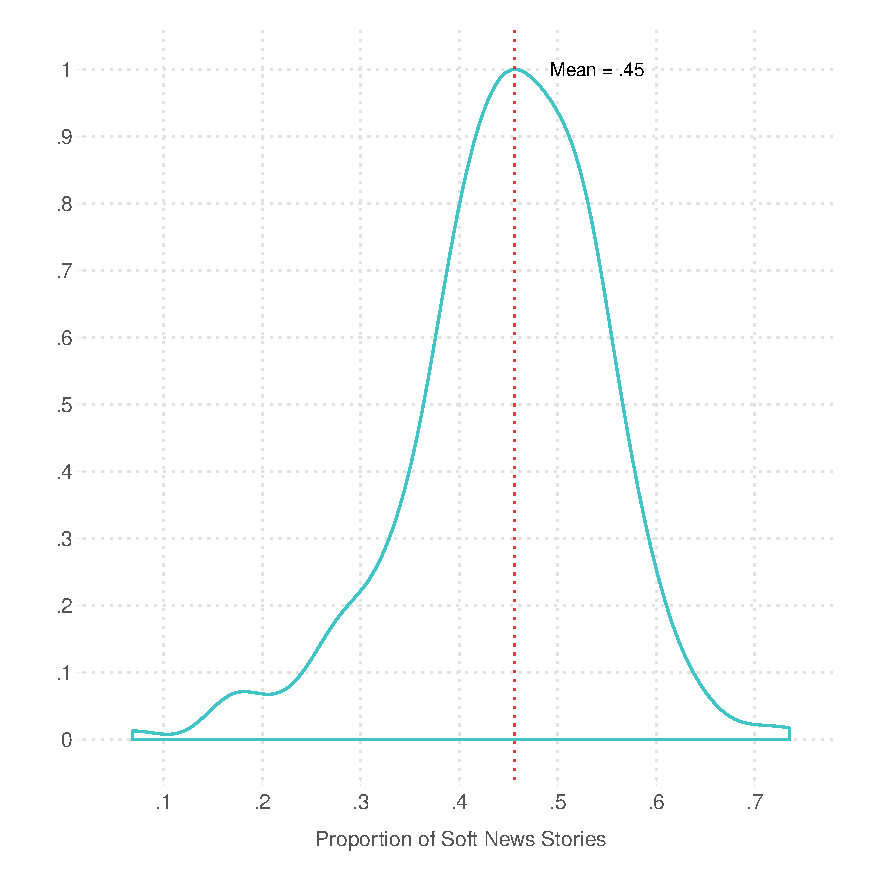
\includegraphics[scale=.9]{../figs/prop_soft_news_by_domain.pdf}
\label{fig:agg_density_domain}
\end{figure}

\end{document}
